\section{Additional Simulation Detail}
\label{app:extra-sim}

This appendix gives further detail behind the robustness checks summarized in Sections~\ref{sec:regulator} and~\ref{sec:calibration}.

\subsection{Robustness of the Regulator's Threshold to Compliance Costs}

The objective~\eqref{eq:regulatorobjective} counts only long-run quality, not the firm's investment spending, so a natural worry is that Section~\ref{sec:regulator}'s recommendation is an artifact of ignoring cost: perhaps a stricter $\tau$ only looks attractive because it hides an ever-rising compliance burden. We check this directly, tracking the long-run time-averaged investment rate $\mathrm{Cost}(\tau)$ alongside $W(\tau)$ across the same $\tau$-sweep (Figure~\ref{fig:costwelfare}). At both boundaries of Case (b) — $\tau \to q^*(p_L)^+$ and $\tau \to q^*(p_H)^-$ — the cycle degenerates and $\mathrm{Cost}(\tau)$ converges to the same value, the drift-offsetting rate $c_\delta$ common to every steady state of the model; in between, cycling amplitude is largest and $\mathrm{Cost}(\tau)$ rises above $c_\delta$, peaking around $\tau\approx0.70$--$0.75$ at roughly $38\%$ above $c_\delta$ before falling back. Contrary to the natural first guess that cost rises monotonically alongside quality as $\tau$ tightens, cost is instead \emph{hump-shaped}: cycling amplitude, not the threshold's strictness per se, drives excess investment, since a shallow cycle near either edge of Case (b) keeps both phases close to the drift-offsetting rate, while a wide cycle in the interior forces larger swings between over-investing while exposed and under-investing while certified.

This shape has a direct consequence for any cost-adjusted objective $W_c(\tau) = W(\tau) - \kappa\,\mathrm{Cost}(\tau)$, $\kappa\geq0$: because $\mathrm{Cost}(\tau)$ returns to essentially the same value at $\tau\to q^*(p_H)^-$ as at $\tau \to q^*(p_L)^+$, while $W(\tau)$ is strictly higher at the former, the upper boundary of Case (b) weakly dominates the lower one on cost while strictly dominating it on quality — for \emph{every} $\kappa$, not a specific one. A numerical sweep over $\kappa\in[0,1000]$ confirms $\arg\max_\tau W_c(\tau)$ remains at the top of the achievable range throughout; we did not find a $\kappa$, however large, that produces an interior optimum under this calibration. The corner-solution recommendation of Proposition~\ref{prop:flatregions} therefore appears robust to pricing in compliance cost here — not because cost is negligible in the interior of Case (b), but because its hump shape happens to vanish at exactly the point quality is maximized.

\begin{figure}[t]
\centering
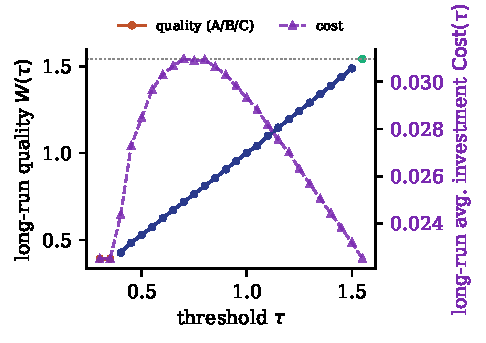
\includegraphics[width=0.55\linewidth]{figures/fig_costwelfare.pdf}
\caption{Long-run quality $W(\tau)$ (left axis) against long-run average investment $\mathrm{Cost}(\tau)$ (right axis), $\rho=0.30$ fixed. Cost is hump-shaped within Case (b), returning to the drift-offsetting rate $c_\delta$ at both boundaries while quality is monotonically higher at the upper one.}
\label{fig:costwelfare}
\end{figure}

\subsection{Calibrating to Real Audit Disclosures: Further Detail}

NYC Local Law 144 has required annual bias audits since July 2023, so real compliance-disclosure data now exists. We do not have, and as we discuss in Section~\ref{sec:discussion}, no one yet has, a firm-level panel suitable for testing the kink or cycling predictions directly, but the disclosures that do exist can ground the plausibility of our parameterization rather than leave $\tau = 0.80$ and the qualitative shape of the trajectories purely stylized.

Two independent field studies give the relevant statistics, and they are in some tension with each other, which we note rather than paper over. Wright et al.~\cite{wright2024null} collected 386 impact-ratio measurements from the disclosures posted by a self-selected subset of 391 covered NYC employers in late 2023 and found 96\% exceeded $0.8$, with 20\% of values missing (concentrated in smaller demographic groups). Gerchick et al.~\cite{gerchick2025auditing} extended data collection from July 2023 through November 2024 and report a substantially larger below-threshold share: 53\% of audits contained at least one impact ratio below $0.8$, and 23\% of group-level results fell below $0.8$ (rising to a bound of 28\% under conservative treatment of missing data). Differences in sampling window, unit of analysis (report-level versus group-level), and treatment of missing data likely explain most of the gap between the two studies' below-threshold shares; we do not have a way to adjudicate between them with currently available data. Gerchick et al. additionally report that reported ratios cluster tightly at or just above $1.0$ with a thin left tail; this is clustering at demographic parity, a full $0.2$ above $\tau=0.80$, not clustering at the legal threshold itself, so it speaks to firms' general performance level rather than directly to our model's predicted bunching around $\tau$. What the combined evidence does support is qualitatively looser: a nontrivial share of employers (Gerchick et al.'s 23--28\%) report ratios below $0.8$, which is inconsistent with a population made up entirely of Case A firms (which, once certified, remain at or above $\tau$ in steady state) and more consistent with a population that includes Case B firms cycling around $\tau$, caught below it depending on the audit date. This gives an empirical anchor for treating $\tau = 0.80$ as the economically relevant threshold in our simulations, rather than an arbitrary modeling choice.

We stop short of a stronger claim. Gerchick et al. identify only 13 audit reports with results in both 2023 and 2024, the entire currently-documented same-employer repeat-disclosure set, and document that employers frequently overwrite prior-year disclosures at the same URL rather than preserving them, that no tool-version identifiers are recorded (so a change in reported ratio cannot be attributed to drift versus re-audit of a modified system), and that only a small, self-selected fraction of covered employers post any audit report at all. These are exactly the obstacles that make a staggered-adoption or event-study test of Theorem~\ref{prop:recurring}'s predictions infeasible with currently available data, as flagged in Section~\ref{sec:discussion}'s limitations; a calibration exercise anchored on cross-sectional distributions is what the current data supports, and it is what we report here.
